\section{Vierleitermessung}

\begin{frame}{Vierleitermessung}
Wieso?
\begin{center}
Bietet die Möglichkeit einer Niedrigohmmessung
\end{center}
\end{frame}

\begin{frame}{Vierleitermessung - Funktionsweise}
 \begin{columns}
   \begin{column}{0.49\textwidth}
  \begin{figure}
    \centering
    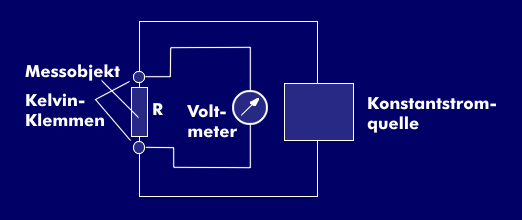
\includegraphics[width=0.7\textwidth]{bilder/vierleiter.png}
    \caption{Schmeatischer Aufbau einer Vierleitermessung}
    \label{fig: versuchsaufbau}
  \end{figure}
\end{column}
\begin{column}{0.49\textwidth}
  \begin{itemize}
    \item {hochohmiger Widerstand am Spannungsmessgerät \\
          $\Rightarrow$ kein Spannungsabfall \\ \hfill }
\item{ mit dem Ohmschengestz kann dann der unbekannte Widerstannd bestimmt werden:
\begin{equation*}
  R=\frac{U}{I}
\end{equation*}}
\end{itemize}
\end{column}
\end{columns}
\end{frame}
